% 
%jff-notes
%
\documentclass[11pt]{article}
\usepackage[pdftex]{graphicx}
\usepackage{amssymb}
\usepackage{latexsym}
%\usepackage{relsize}
\usepackage{textcomp}
%processed for 10 pt 
%\documentstyle[epsf,psfig]{article}
%\documentstyle[epsf]{article}
\oddsidemargin 0pt
\topmargin -0.0cm
\textwidth 6.2in
\textheight 8.5in
\baselineskip 18pt
%\renewcommand{\baselinestretch} {1.5}
\newenvironment{nitemize}
   {\begin{list}{\begin{math}\bullet\end{math}}%
      {\setlength{\leftmargin}{5mm}
       \setlength{\topsep}{1mm}
       \setlength{\parsep}{0in}
       \setlength{\itemsep}{.7mm}}}%
   {\end{list}}

\newcommand{\fract}[2]{\frac{\textstyle #1}{\textstyle #2}}
\newcommand{\trans}[3]{#1 \stackrel{#2}{\longrightarrow} #3}
\newcommand{\notrans}[3]{#1 \stackrel{#2}{\not\! \longrightarrow} #3}
\bibliographystyle{plain}
\begin{document}
\title{An SDRuno plugin for FT* decoding (V2.2)}
\author{
Jan van Katwijk\\
Lazy Chair Computing \\
The Netherlands\\
{\em J.vanKatwijk@gmail.com}}
%\date{}
\maketitle
%\baselineskip 22pt
\ \\
\ \\
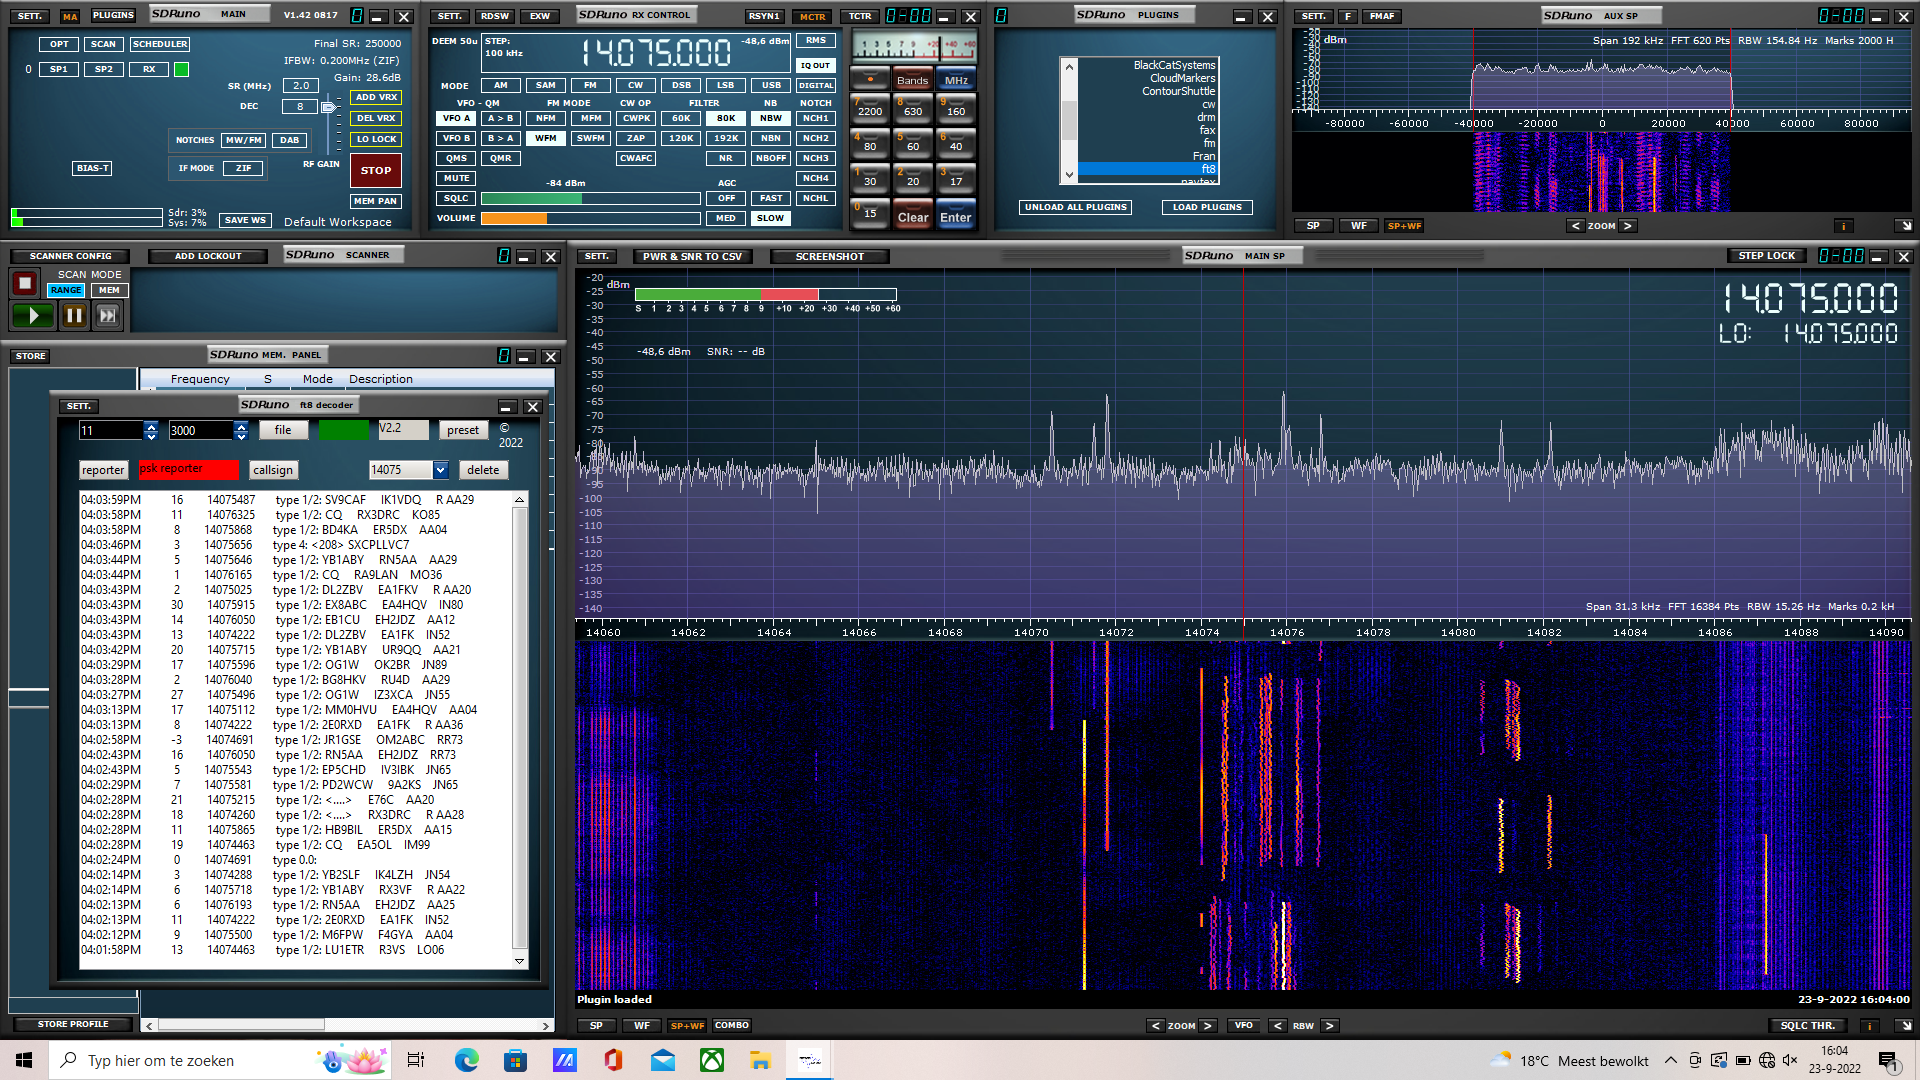
\includegraphics[width=170mm]{SDRunoPlugin_ft8.png}
\ \\
\section{Introduction}
The FT8 plugin is a plugin for decoding FT8 messages and
showing the decoded messages. The plugin is experimental in the sense
that its development is going on.
\par
The plugin - as a community plugin - can be installed by placing it
in the folder for community plugins. Ask SDRplay.com where the folder 
need to be placed on your system, on my system the folder can be found as
subfolder in "Documenten".

\section{Selecting a samplerate}
The plugin uses the IQOUT option of the SDRuno platform. This
output is 192000 samples per second. The plugin itself will reduce
the samplerate to 12000 (and filter accordingly).
The plugin - when started - will do the selection of the IQOUT port.
\par
The default setting for SDRuno (at least with me) is that the input samplerate
is 2 MHz, and the main spectrum display will show a spectrum of the full 2 MHz.

\begin{figure}[htp]
\centering
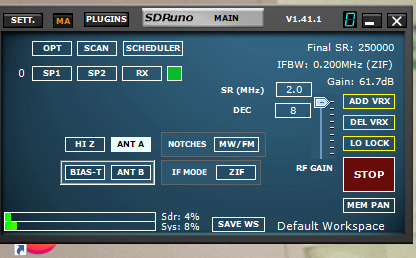
\includegraphics[width=80mm]{uno-main-widget.png}
\caption{ft8Plugin: uno widget}
\label{figure:freq_select}
\end{figure}

It is useful to zoom in in the spectrum, after all
the spectrum of the region of interest is only a few KHz wide.
\section{The FT8 plugin and the reporter map}
\begin{figure}[htp]
\centering
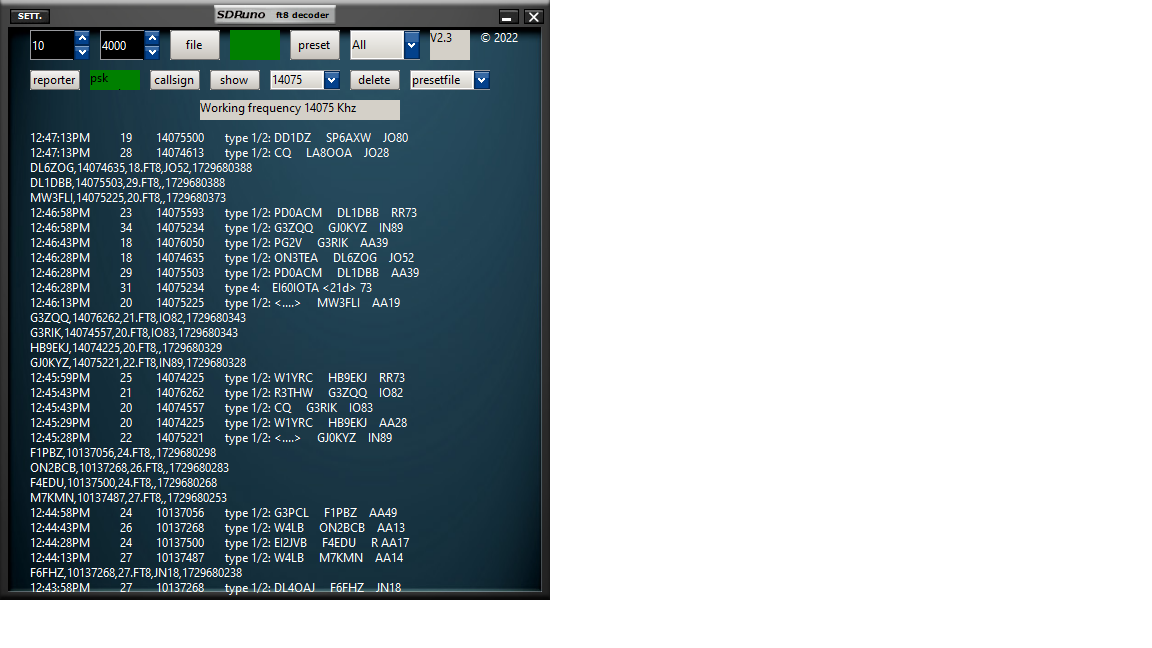
\includegraphics[width=170mm]{ft8-widget.png}
\caption{ft8Plugin: the widget}
\label{figure:ft8_widget}
\end{figure}
\par
The widget for the FT8 plugin is straight forward and does not have a lot
of controls.
On top there are two lines with buttons and some info,
and there is a larger space where the text of the messages received is written.
\par
On start up the white box will show the callsign and the grid of the
receiver - obviously only if specified\footnote{If no callsign and grid are
specified no data will be transmitted to the pskreporter site.}.
Then it will show for each decoded FT8 message a few fields
\begin{itemize}
\item
the time of decoding the message;
\item
the strength of the FT8 message, relative to the average signal
strength during reception of the FT8 message;
\item the frequency of the message with an accuracy of 3.125 Hz (tone
distance is 6.25 Hz);
\item the message type;
\item the message itself.
\end{itemize}

On the top  line in the control part of the widget there are
two selectors and three buttons
\begin{itemize}
\item
The {\em first} selector sets the value for the number of iterations,
to be applied in the LDPC decoding. Higher values
{\em may} lead to better decoding but are expensive in terms of CPU load.
Default value is 10, which should be enough for.
A selected value will be stored and used the
next invocation of the plugin.
\item
 the {\em second} selector sets the bandwidth within the spectrum
in which ft8 messages are searched for.
Default value is 2 KHz, maximum is 6 MHz.
The selected frequency is here the {\em center} frequency, so a
width of 4 KHz means from -2 KHz to +2 KHz wrt the selected frequency.
{\em Obviously, the larger the width, the more processing power is needed.}
\item
Next a button labeled {\em file} is there. As the name suggests, a file can
be selected in which the data is stored. If the data is being written the
label next to the button will be colored red, if no data is written the color
of the label will be green.
\item the second button on the first row is labeled {\em preset}. The plugin 
supports a number of preset frequency values. In previous versions this was a
static list, in this version the user can add his/hers preferred frequencies
to the list (and the default list is shortened).
\item The button labeled {\em All} allows selection in the displayed messaged
between all decoded messages or just the "cq" messages.
\item to the far right of the top line there is the inevitable copyright symbol.
\end{itemize}
The second line in the widget shows three (or four) buttons, a label
and a combobox
\begin{itemize}
\item the button with the label {\em reporter} can be used to switch
the {\em PSKReporter} on or off. The state is reflected in the label,
{\em green} indicates that the reporter is "on", otherwise the label
will color {\em red}.
\item the PSK reporter sends the data to the server 
{\footnotesize
\begin{verbatim}
"https://www.pskreporter.info/pskmap.html
\end{verbatim}
}
In order for the pskReporter info site to show the "monitor",
i.e. data of the receiver that sends the messages, the ft8 plugin
sends some information on the "home" station, a.o. a callsign and the 
grid location to the pskreporter.
The button {\em callsign}, when touched, shows a widget
where a callsign and a grid can be entered. Values will be maintained
between invocations of the plugin.
\item if the psk report function is selected, a third button shows,
labeled "show". If touched, the ft8 plugin shows the elements of
the messages  that are transmitter to the psk reporter.
The picture shows these messages.
Transmission takes place in UDP mode, using port 4739 of the pskreporter server.
\item FT8 is transmitted is well defined regions in different amateur bands. To
ease  switching between these bands, the plugin now contains a button - labeled
- {\em presets} where one may select among a list of frequencies, known to
be in these regions. By default the list merely contains four of five
frequencies (of course the one I am using most of the time), and as said,
your own preferred frequencoes can be added to the list.
Of course, the added frequencies will be saved between sessions.
\item the {\em delete} button will remove the last entered preset frequency.
\item A user-defined {\em preset} file can be used.
\end{itemize}
The third row consists of a single label, showing the selected working frequency.
\begin{figure}[htp]
\centering
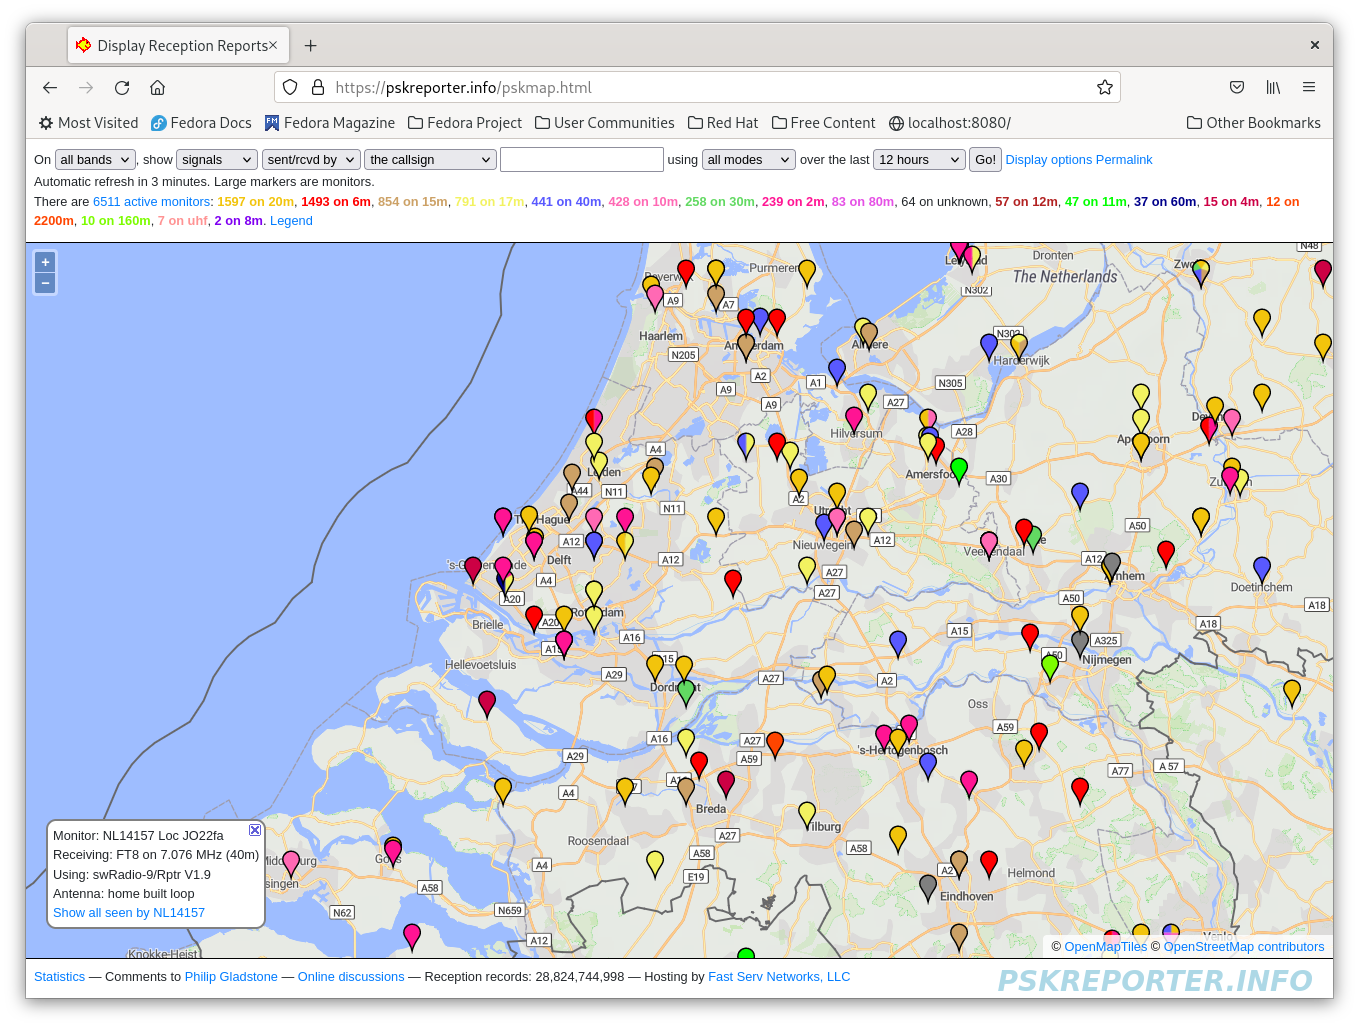
\includegraphics[width=140mm]{pskreportermap.png}
\caption{ft8Plugin: the map, example}
\label{figure:pskReportermap}
\end{figure}
\par
The widget will show up to 30 of the last received messages. Of course
all messages are saved in a file whenever a file is selected

\begin{figure}[htp]
\centering
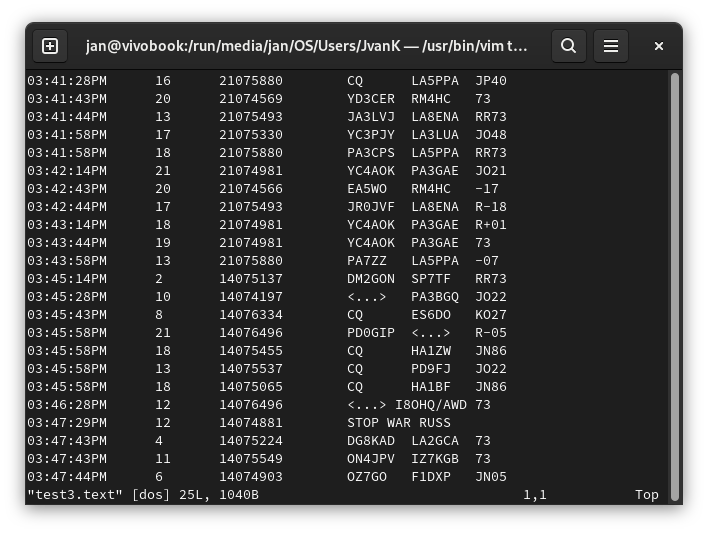
\includegraphics[width=100mm]{ft8-file.png}
\caption{ft8Plugin: file output}
\label{figure:ft8_file}
\end{figure}
\section{A note on FT8 decoding}

FT8 decoding is essentially based on a - more or less - "intelligent"
brute force approach (sounds like a "Contradictio in terminis").
In a first step an attempt is made to preselect 
"potentials", i.e. potential messages based on matching the
input with a costas array of 7 tones.
\par
In the second step for each of these potentials an LDPC based
error detection/recovery mechanism is applied. First the 79 subsequent
tones are collected, the 58 data tones are mapped upon 174
soft bits (3 bits per tone) and the LDPC algorithm is asked
to make that into "hard" bits.
Finally, in a third step the resulting message is subjected to
a CRC check.
If the check succeeds the bits are translated into a message.
\par
Note that the parameters in the first stage may be too strict,
and not all messages are in the set of potentials, or they may be too loose,
and the set of potentials is too large. Some criteria have to be applied to
do the selection, but it is not obvious that a single set of criteria
is optimal under all circumstances.
\par
An encoded FT8 message is 91 bits (including the CRC),
and 83 error correction bits are appended.
Of course, the probability that on receiving a transmission, the 
error correction bits contain - roughly - the same amount of errors
as the message bits is pretty large.
\par
The net effect is that the result of the application of the error correction
may be that incoming garbage is transformed to something resembling a
message, and the other way, a correct message may suffer from
errors in the error correction bits and may be transformed into
garbage. A CRC check is therefore absolutely needed.
\par
Anyway, the decoder may - and probably will - miss some messages
in the transmitted band,
and I am still looking for the "best" parameter settings for the
different functions.
\section{Future work}
Current work is on optimizing 
parameter settings and extending the encoding.
Detecting potential messages requires finding detecting peaks in the spectrum
where the amplitude value is (relatively) large, compared to its environment.
While that sounds easy, there is a pretty large "noise" component,
and parameters for detecting very small peaks are not always capabel of
detecting large peaks.
\par
In the current version an attempt is made to decode all message types,
however, messages in some message types need further processing.
\par
Further work is required to extract all calls that can be send to the PSKreporter.
\section{Copyright and acknowledgments}

The code in the plugin uses parts of the code of the FT4FT8 decoding
software of Karlis Goba.
Especially the LDPC decoder is (almost) a copy of his code, and the copyright
to the parts taken or derived from his code are gratefully acknowledged.

The copyrights of the code of the plugin - not covered by the above -
is by me.
The software is available under a GPL V2.
Note that under this license you are free to use the plugin, and
I will make the source available to you on request,  but the software is provided "as is",
and no garantees are given that the software meets your requirements.
\par
Note that - as the title of this document states - the plugin is still
experimental, implying that the search for optimal parameter settings continues.
\end{document}


